\subsection{Sicherheit}
In diesem Kapitel geht es darum, wie wir uns vor zugriffen von außen schützen wollen. 
Dazu schauen wir uns an, welche Sicherheitsvorkehrungen wir sowohl im Frontend als auch 
im Backend getroffen haben.

\subsubsection{Frontend}
Im Frontend ist Keycloak so konfiguriert, dass man sich dort einloggen kann, wenn man möchte. 
Um die Seite des Chats aufrufen zu können muss man nicht eingeloggt sein. 
Anders sieht das beim Admin-Interface aus. 
Möchte man auf das Admin-Interface zugreifen, so muss man sich zuerst einloggen. 
\begin{figure}[H]
    \centering
    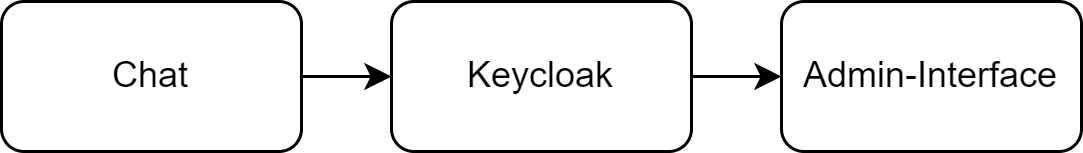
\includegraphics[width=0.8\textwidth]{bilder/technologien/frontend-sicherheit.png}
    \caption{Frontend-Sicherheit}
    \label{fig:Frontend_Sicherheit}
\end{figure}
\noindent Kommt man jetzt noch nicht in den Admin-Bereich, dann hat wohl der benutzte Account nicht die benötigten Rechte. 
Jedem Account sind Rollen zugeordnet, wie zum Beispiel ''Admin'', ''Student'' und ''Professor''. 
Nur wenn man mit einem Account, welcher die Admin-Rolle besitzt eingeloggt ist, kann auf das Admin-Interface zugreifen.

\subsubsection{Backend}
Für das Backend ist Keycloak so konfiguriert, dass man sich nicht einloggen kann. 
Es dient nur zur Verifizierung von Tokens. 
Geschützt ist jeder mögliche Request an unsere Rest-API. 
Bei jeder Anfrage an die Rest-API muss ein valider Security Bearer Token im Header mitgeschickt werden. 
Ist dies nicht der Fall, so wird die Anfrage sofort abgelehnt. 
Sollte ein Token vorhanden sein, wird dieser vom Keycloak-Server geprüft. 
Ist der Token valide wird geprüft, ob der Nutzer, zu dem dieser Token gehört, 
über die nötigen Rollen verfügt. 
So kann auch niemand ohne gültigen Token zu einem Admin-Account über die Rest-API auf unsere Daten zugreifen, 
sie löschen oder ändern. 
Bei einer Anfrage vom Frontend wird automatisch der aktuelle Token des eingeloggten Nutzers mitgeschickt.

\newpage
\subsubsection{Angriffs-Szenarios}
\noindent \textbf{Szenario 1: API}
\newline
Ein Angreifer findet die Pfade zu unserer Rest-API heraus. 
Mithilfe dieser Information möchte er Zugriff auf unsere Daten in der Datenbank erlangen.
\newline \newline
\noindent \textbf{Lösung: } \newline
Da der Angreifer aber keinen gültigen Security Token hat, den er mitschicken kann, ist es ihm 
nicht möglich eine Anfrage an die API zu stellen.
\newline \newline

\noindent \textbf{Szenario 2: API mit Token}
\newline
Der Angreifer hat einen gültigen Token in die Hände bekommen und sendet diesen nun mit in der Anfrage.
\newline \newline
\noindent \textbf{Lösung: } \newline
Selbst wenn der Token zu einem Account mit der Admin-Rolle gehören sollte, so muss der Angreifer 
sich trotzdem sehr beeilen, da die Token regelmäßig in kurzen Abständen erneuert werden.
\newline \newline

\noindent \textbf{Szenario 3: Admin-Interface}
\newline
Der Angreifer möchte sich Zugang zum Admin-Interface verschaffen, indem er den Login-Prozess 
überspringt und direkt auf einen Pfad des Admin-Interfaces zugreift. 
\newline \newline
\noindent \textbf{Lösung: } \newline
Da jeder Pfad des Admin-Interfaces durch Keycloak geschützt ist, wird für jeden Pfad 
einzeln geprüft, ob der Nutzer die nötigen Rechte besitzt.